\documentclass[a5paper,twoside,11pt,openany]{book}

%%%%%%%%%% Packages %%%%%%%%%%
\usepackage[outer=2cm, inner=2cm, bottom=2.5cm, footnotesep=1cm]{geometry}
\usepackage[super]{nth}
\usepackage[bottom]{footmisc} 
\usepackage{longtable}
\usepackage{fancyhdr}
\usepackage{graphicx}
\usepackage{wrapfig}
\usepackage{enumitem}
\usepackage{fontspec}
\usepackage[german,greek,english]{babel}
\languageattribute{greek}{ancient} 
\usepackage{epigraph}
\usepackage{afterpage}
\usepackage{nonumonpart}
\usepackage{titlesec}
\usepackage{microtype}
\usepackage{titling} 
\usepackage[LGR,T1]{fontenc}
\usepackage{bold-extra}
\usepackage{listings}
\usepackage[svgnames]{xcolor} 
\usepackage{libertine}
\linespread{1.1}
\usepackage[nopbinverse,nocritical,noend,noeledsec,nofamiliar,noledgroup]{reledmac}
\usepackage[]{reledpar}
\usepackage[font=small,labelfont=bf]{caption}
\usepackage{xhfill}
\definecolor{rulecolor}{rgb}{0.34, 0.01, 0.1}
\usepackage[hyphens]{url}
\usepackage{xurl}
\usepackage{moreenum}
\usepackage{tocloft}
\usepackage{teubner}
%\usepackage{draftwatermark}
\setlength{\cftbeforechapskip}{0.5em}
\setlength{\cftchapnumwidth}{5em}
\usepackage{ccicons}
\usepackage{metalogo}
\usepackage{epigraph}
\usepackage{Zallman,lettrine}
\usepackage{datetime}


\newdateformat{monthyeardate}{%
  \monthname[\THEMONTH] \THEYEAR}

\newfontfamily{\PHtitl}{Philokalia}[
  %Renderer=OpenType,
  Script=Greek,
  Style=TitlingCaps,
  Scale=0.3,
]

\newenvironment{doubletitle}
{
\thispagestyle{empty}
}

\newlength{\drop}

\raggedbottom
\makeindex

\renewcommand\UrlFont{\itshape}

\cftpagenumbersoff{part}

%\SetWatermarkText{Preview}
\newlength\longest
\setlength{\marginparwidth}{0pt}
\setlength{\headheight}{15pt}

\titleformat{\chapter}[display]
{\filcenter}{\mbox{}\xrfill[0.4ex]{3pt}[rulecolor]\textsc{\large\enspace\chaptername \thechapter}\enspace\xrfill[0.4ex]{3pt}[rulecolor]\mbox{}}{0.3ex} {{\color{rulecolor}\titlerule[1pt]}\vskip3ex\huge\bfseries}[\medskip{\color{rulecolor}\titlerule[1pt]}]

\titleformat{\section}[wrap]
{\normalfont\bfseries}
{\thesection.}{0.5em}{}
\titlespacing{\section}{12pc}{1.5ex plus .1ex minus .2ex}{1pc}

\addto\captionsgreek{\renewcommand{\chaptername}{Κεφάλαιον }}
\addto\captionsenglish{\renewcommand{\chaptername}{Chapter }}
\renewcommand{\thechapter}{\Roman{chapter}}

%%%%%%%%%% Fancy HDR %%%%%%%%%%
\pagestyle{fancy}
\fancyhf{}
\fancyhead[LE,RO]{\thepage}
\fancyhead[LO]{\textsc{\nouppercase{\leftmark}}}
\fancyhead[RE]{\textsc{\shorttitle}}
\fancypagestyle{plain}{
\fancyhf{} 
\fancyhead[LE,RO]{\thepage}
\fancyhead[LO]{\textsc{\nouppercase{\leftmark}}}
\fancyhead[RE]{\textsc{\shorttitle}}}

%%%%%%%%%% Greek Dates %%%%%%%%%%
\newcommand\greekdate[1]{%
  \ifcase#1\relax
  \or
    \uppercase{Γαμηλιών}
  \or
    \uppercase{Ἀνθεστηριών}
  \or
    \uppercase{Ἐλαφηβολιών}
  \or
    \uppercase{Μουνιχιών}
  \or
    \uppercase{Θαργηλιών}
  \or
    \uppercase{Σκιροφοριών}
  \or
    \uppercase{Ἑκατομβαιών}
  \or
    \uppercase{Μεταγειτνιών}
  \or
    \uppercase{Βοηδρομιών}
  \or
    \uppercase{Πυανεψιών}
  \or
    \uppercase{Μαιμακτηριών}
  \or
    \uppercase{Ποσειδεών}
  \else
     \uppercase{Error}
  \fi
}

%%%%%%%%%% Titles %%%%%%%%%%
\newcommand{\shorttitle}{The Gospel of John}
\title{The Gospel of John: A Modern Translation with Notes and the Original Greek Text}

%%%%%%%%%% Document begin %%%%%%%%%%
\begin{document}
\frontmatter
\pagenumbering{gobble}
\pagestyle{empty}

%%%%%%%%%% Half-title %%%%%%%%%%
\thispagestyle{empty}
\begin{center}
	\hspace{0pt}
	\vfill
	\drop=0.1\textheight
    \centering
    \vspace*{\baselineskip}
    \rule{\textwidth}{1.6pt}\vspace*{-\baselineskip}\vspace*{2pt}
    \rule{\textwidth}{0.4pt}\\[\baselineskip]
    {\LARGE THE GOSPEL \\ OF \\[0.3\baselineskip] JOHN }\\[0.2\baselineskip]
    \rule{\textwidth}{0.4pt}\vspace*{-\baselineskip}\vspace{3.2pt}
    \rule{\textwidth}{1.6pt}\\[\baselineskip]
    \vfill
\end{center}

%%%%%%%%%% Title page %%%%%%%%%% 
\begin{doubletitle}
    \drop=0.1\textheight
    \centering
    \vspace*{\baselineskip}
    \rule{\textwidth}{1.6pt}\vspace*{-\baselineskip}\vspace*{2pt}
    \rule{\textwidth}{0.4pt}\\[\baselineskip]
    {\LARGE THE GOSPEL \\ OF \\[0.3\baselineskip] JOHN }\\[0.2\baselineskip]
    \rule{\textwidth}{0.4pt}\vspace*{-\baselineskip}\vspace{3.2pt}
    \rule{\textwidth}{1.6pt}\\
    
    \scshape
    \rule{\textwidth}{0.4pt}\\[\baselineskip]
    {\Large Volume II of the New Testament \\ Translation Series }\\[0.2\baselineskip]
    \rule{\textwidth}{0.4pt}\vspace*{-\baselineskip}\vspace{3.2pt}\\[\baselineskip]\vspace*{2\baselineskip}
    
    A Modern Translation with Notes \\
    and the Original Greek Text \\
    \vspace*{2\baselineskip}
    Edited and Written by \\[\baselineskip]
    {\Large Marvin Johanning\par}
    \vfill
    {\scshape \monthyeardate\today} \\
    {\large Marvin Johanning}\par
\end{doubletitle}

%%%%%%%%%% Title page Greek %%%%%%%%%% 
\begin{doubletitle}
    \drop=0.1\textheight
    \centering
    \vspace*{\baselineskip}
    \rule{\textwidth}{1.6pt}\vspace*{-\baselineskip}\vspace*{2pt}
    \rule{\textwidth}{0.4pt}\\[\baselineskip]
    {\uppercase{\LARGE Τὸ εὐαγγέλιον \\ κατὰ \\[0.3\baselineskip] Ἰωάννην }}\\[0.2\baselineskip]
    \rule{\textwidth}{0.4pt}\vspace*{-\baselineskip}\vspace{3.2pt}
    \rule{\textwidth}{1.6pt}\\
    
    \scshape
    \rule{\textwidth}{0.4pt}\\[\baselineskip]
    {\Large\uppercase{Τόμος δεύτερος τῇ συλλογῇ \\ τῶν τῆς Καινῆς Διαθήκης μεταφράσεων } }\\[0.2\baselineskip]
    \rule{\textwidth}{0.4pt}\vspace*{-\baselineskip}\vspace{3.2pt}\\[\baselineskip]\vspace*{2\baselineskip}
    
    \uppercase{Μετάφρασις καινὴ ὑπομνήμασι \\
    καὶ δὴ καὶ τοῖς ἀρχαῖοις Ἑλληνικοῖς λόγοις} \\ 
    \vspace*{2\baselineskip}  
    \uppercase{Τοῦτο τὸ βιβλίον ἐγράφη ὑπὸ τοῦ \\[\baselineskip]
    {\Large Κλεοφίλου τοῦ Ἰωάννου}}\par
    \vfill
    {\scshape \uppercase{\greekdate{\the\month} τοῦ} \Greeknumeral{\the\year}} \uppercase{ἔτους}  \\
    {\large \uppercase{Κλεόφιλος τοῦ Ἰωάννου}}\par
\end{doubletitle}

%%%%%%%%%% Copyright and Impressum %%%%%%%%%%
\thispagestyle{empty}
\vspace*{\fill}
\noindent\textsc{\underline{Text}}: © Copyright \the\year{} Marvin Johanning

\noindent\textsc{\underline{Greek text}}: Eberhard Nestle's ``Novum Testamentum Graece'', 1904


\noindent\textsc{\underline{Printing and Publishing}}: BoD – Books on Demand, Norderstedt
\noindent\textsc{\underline{ISBN}}: 978-3-XXXX-XXXX-X

\bigskip

\noindent© \the\year{} by Marvin Johanning \ccbyncnd\\``\thetitle'' by Marvin Johanning is licensed under CC BY-NC-ND 4.0. To view a copy of this license, visit \url{https://creativecommons.org/licenses/by-nc-nd/4.0}.\\This copyright statement applies neither for the images and illustrations found in this book nor for the Ancient Greek text; these are all in the public domain and can be used freely.

\vspace{30mm}
\noindent\fbox{%
    \parbox{\textwidth}{%
    \noindent\foreignlanguage{german}{Bibliografische Information der Deutschen Nationalbibliothek: Die Deutsche Nationalbibliothek verzeichnet diese Publikation in der Deutschen Nationalbibliografie; detaillierte bibliografische Daten sind im Internet über \url{dnb.dnb.de} abrufbar.}
    }%
}
\newpage
\thispagestyle{empty}
  \mbox{}
  \newpage

%%%%%%%%%% Introductory quote %%%%%%%%%%
\clearpage
\thispagestyle{empty}
\null\vfill
\settowidth\longest{\huge\uppercase{Καὶ εἶδον οὐρανὸν καινὸν}}
\begin{center}
\parbox{\longest}{%
  \raggedright{\huge%
    \uppercase{Μακάριος ὁ ἀναγινώσκων καὶ οἱ ἀκούοντες τοὺς λόγους τῆς προφητείας καὶ τηροῦντες τὰ ἐν αὐτῇ γεγραμμένα.} \par\bigskip
  }
  \raggedleft\Large\MakeUppercase{Rev. 1:3}\par%
}
\vfill\vfill
\clearpage\newpage
\end{center}
\newpage
\thispagestyle{empty}
  \mbox{}
  \newpage

%%%%%%%%%% Table of Contents %%%%%%%%%%
\thispagestyle{empty}
\tableofcontents
\newpage
\thispagestyle{empty}
  \mbox{}
  \newpage
  
%%%%%%%%%% Introduction and Preface %%%%%%%%%%
\thispagestyle{empty}
  \mbox{}
  \newpage
\part*{\textsc{Preface}}
	\markboth{Preface}{Preface}
	\addcontentsline{toc}{part}{Preface}

\pagestyle{fancy}
\pagenumbering{roman}
%%%%%%%%%%% The New Testament Translation Series %%%%%%%%%%
\chapter*{The New Testament Translation Series \\ \large General introductory information about the series}
  \markboth{The New Testament Translation Series}{The New Testament Translation Series}
  \addcontentsline{toc}{chapter}{The New Testament Translation Series}
%%%%%%%%%% Introduction %%%%%%%%%%
\chapter*{The New Testament Translation Series \\ \large General introductory information about the series}
  \markboth{The New Testament Translation Series}{The New Testament Translation Series}
  \addcontentsline{toc}{chapter}{The New Testament Translation Series}
  
This book is the second part in The New Testament Translation Series — henceforth referred to simply as the NTTS for simplicity's sake — which is my attempt at a modern, yet still faithful to the original manuscripts, translation of the New Testament. The previous part contained my translation — with a vast amount of related illustrations and paintings — of the Revelation (or Apocalypse) of John and marked the beginning of the series. 

This second part of the series contains fewer illustrations, due to the fact that imagery of the gospels is far less vivid than that of the Revelation, but my method of translating the original text has remained the same. Thus, if you are already familiar with my translations, you can skip this section; if you, however, do not and wish to gain further insight into how I translate texts, I encourage you to continue reading. 
  
Translations of the New Testament are plentiful — indeed, the vast majority of translations one can attain nowadays are much more professionally made and have had dozens of people working for hundreds upon hundreds of hours perfecting them. Therefore, it may come as a surprise to some that I — someone who has written what you are about to read in his free-time and who has never “professionally” studied Ancient Greek — would take it upon myself to write my own translation of one of the books of the New Testament. 

Thus, in order for you to understand why this particular translation exists and how it differs from other translations, I decided to write this introduction, detailing not only the philosophy behind the manner in which I translate texts, but also the recommended ways of reading my translation. 

\section*{Textual basis}
  \addcontentsline{toc}{section}{Textual basis}
As I do not have access to a large amount of funds, I was required to use a textual basis published in the public domain. Thankfully, a substantial amount of editions of the Greek New Testament are now available in the public domain, which means that there is not a shortage of texts to utilise; finding a digital edition of such a public domain text — that is itself in the public domain — was, however, a slightly more complicated task to accomplish. 

As luck would have it, however, a very kind man going by the name of Diego Santos has digitised the 1904 edition of Eberhard Nestle's \textit{Novum Testamentum Graece} and published it on his website (\url{https://sites.google.com/site/nestle1904/home}) in the public domain.

Without the tremendous amount of effort he put into the digitisation of Nestle's 1904 edition, I would not have been able to produce this book. And whilst there have been a great number of revised editions of his work (as of \today, the most recent one is NA28, i. e. the \nth{28} edition), the changes are minor enough for me to look past them. 

\section*{Cultural issues}
  \addcontentsline{toc}{section}{Cultural issues}
  
 Translating texts from another language is never as straight-forward as some people might believe; one cannot simply pick up a dictionary, start translating and expect to have a coherent result thereafter. I have met a number of people who sincerely believe that they will be able to study a language by solely learning vocabulary and leaving the acquisition of grammatical concepts to ``intuition''. 
 
 Such approaches are — in my opinion — bound to fail, unless it is one's goal to part-take in a spelling contest in another language (as some people have, indeed, previously done). 
 
 Instead, translating a text requires not only an at least somewhat firm grasp of the language's grammatical concepts — and how they might be translated properly without distorting their meaning too considerably —, but also an understanding of the source text and the cultural background of the people who speak the language being translated from. 
 
 Of the above-mentioned skills, however, only two can be harnessed with relative ease, namely the attaining of a firm understanding of the grammatical concepts of the language and of the text being translated; the latter skill — (somewhat) extensive knowledge of the cultural background of the people who spoke the language — is slightly more difficult.
 
 For, indeed, we are unable to take a time-machine and live with the ancient Greeks — or, in this particular instance, those living at around 200 AD. It is, therefore, much more difficult to get an adequate understanding of the cultural background; yet it is still quite possible to get a decent understanding of it through reading history books and reading original texts from that time.
 
 Another aspect that needs considering is the fact that the general populace is most likely unaware of many of the cultural aspects of the people who lived during the time of the events of the New Testament; it is, therefore, imperative to assume that whoever is reading one's translation is oblivious to many of the cultural terms used in the text.  
 
 The translator must, therefore, consider which terms are to be explained to the reader and which are not; for explaining every single ``strange'' term one encounters could lead to the text containing too much of one's personal opinions and viewpoints. 
 
 Personally, I explain terms which a modern reader might be confused by (such as the Ancient Greek word δηνάριον, which is the equivalent of the modern-day penny), but do not generally explain those terms that might leave the ``uninitiated'' slightly mystified, but which make sense when one knows the basics of the Biblical story.
 
 \section*{Linguistic issues}
  \addcontentsline{toc}{section}{Linguistic issues}
  
Despite my having written that the obtaining of a decent understanding of the grammatical concepts of a language is relatively simple, it is, by no means, truly \textit{simple} — indeed, the word ``relatively'' is of great import in this sentence. This is especially true when it concerns the translating of a text, particularly one that — as you shall see in the chapter hereafter — contains a not insignificant amount of strange linguistic features. 

As the translator, I am forced to consider whether to translate what the original author wrote verbatim, or whether to change its meaning in English to abide by the rules of regular English prose. Frequently, I opt to present the reader with the literal translation and an alternative interpretation (in brackets); a matter I will more fully explain in the \textit{How to read this translation} section later on. 

Indeed, I try staying as close as I possibly can to the base text, as I do not want to ``disturb'' the original \ae sthetics of the prose. Yet, there are times where a literal translation would yield something so bizarre and utterly incomprehensible that a modern English speaker would be greatly mystified by it — and in such instances, I do take the liberty of slightly rephrasing the original sentence, all the while keeping the meaning intact as best I can. 

My particular approach to translation is a more literal one; this is especially true — and, in my opinion, important — when it concerns important documents such as, in this case, a religious text. The wrong translation — or, indeed, interpretation — may lead to an entirely different outcome; and as religious texts are abound in symbolism that is, frequently, open to interpretation, it is my goal to present the reader not with my own, personal world-view, but rather with an undiluted — but still pleasant-to-read — version of the base text in a language he can understand.  

Balancing the ``pleasant-to-read'' aspect of my translation with linguistic accuracy is a rather delicate task, however, and I generally prefer to err on the side of linguistic accuracy. Frequently, some authors of the New Testament books re-use the same phrases, expressions and words in close proximity, which is a practice frowned upon by most English speakers when reading prose; and even though I often have the ability to choose a slightly different word for the sake of diversity, I choose to, instead, — in the vast majority of instances, at any rate — use the same repetition as the original does too. 

\section*{How to read the translation}
  \addcontentsline{toc}{section}{How to read the translation}
  
This translation differs substantially from others you might be used to, for it contains a not insignificant amount of notes within parentheses. This approach might be somewhat perplexing to those who are not used to it and I would, therefore, like to explain how to properly read parenthesised text.  

Indeed, there are, in actuality, several different types of parenthesised text, all fulfilling slightly different functions. In general, it can, however, be said that the text within parentheses contains my own opinions and interpretations that cannot be found in the base text; and as I do not wish to impose my world-view upon the reader — as mentioned earlier —, these personal viewpoints have been placed in brackets to clearly separate them from the base text. 

Should you wish to learn more about the various categories of notes, I shall herein explain them to you. We will begin by covering the ``explanatory type''; this particular category is used to explain strange or unusual text passages or words. An example of this would be the aforementioned ``denarius'' which is followed by an explanatory parenthesis clarifying its modern-day equivalent meaning (i. e. penny / cent). 

Another very frequently-used variety is the ``supplementary type''. This particular variety of parenthesised text is used whenever the author implies a certain meaning, but does not explicitly write it out; or where an additional phrase makes the sentence sound more natural in English. An example of this can be found in my translation of the Apocalypse in II:4-5, where the addition of ``I know'' (``[…] and (I know) that you cannot […] '') clarifies the meaning of the sentence. 

The next category of parenthesised text that we shall explore is the ``alternative reading type''. Anyone who has ever studied a second language for any length of time will be aware of the fact that words can — depending on context — be translated in a variety of ways. Therefore, whenever I felt that a word or phrase could be translated in a different manner, I add that alternative reading in parentheses behind the word or phrase it is referring to. 

Within the alternative reading type, there exists a subset I am unsure what to call — perhaps ``uncertain alternative reading type'' would be an adequate description. Whenever I suspect there could be a possible alternative reading but I am not entirely certain it actually \textit{could} be an alternative reading, I place the alternative text within parentheses and place a question mark thereafter. 

It should now have become evident that there exist a rather large number of notes to be found within parentheses immediately following the sentence, word or expression they are referring to. I have taken great inspiration from, what I would most certainly deem, the most accurate and simply the best German translation of the Bible — The Mengebibel. For, indeed, that particular translation of the — in this particular instance entire — Bible follows a similar style; and as I have found it to be a great pleasure to read, I decided to write something similar in English. 

I highly recommend \textit{always} reading the parenthesised text, as it not only provides the reader with alternative readings and explains terms that might be unknown to him, but it also adds words and phrases that makes the reading much more fluid and pleasant; the translation should, however, be perfectly readable when skipping the parenthesised text, though knowledge of the underlying Greek idioms might be needed in order to properly understand certain passages. 

%%%%%%%%%% Note %%%%%%%%%%
\chapter*{Author's Note  \\ \large On obtaining a copy, compilation and license information}
	\markboth{Author's Note}{Author's Note}
	\addcontentsline{toc}{chapter}{Author's Note}

As this book is not “copyrighted” in the traditional sense, I thought it prudent to write a short informational text here, explaining how you may legally attain your own (free) copy of my work, how you may use it and how to support me. 

First and foremost, it is important to note that I am not making a non-watermarked PDF file of this book freely available; you may, however, at any time, download its source-code and compile it into any format that you wish — this is made possible through my having written this book in \LaTeX. This compilation process requires a full \LaTeX\ installation and a \LaTeX\ compiler compatible with my book, preferably \XeLaTeX\ or Lua\LaTeX; I would, however, strongly advise against the usage of pdf\LaTeX, as the Greek text appears to trouble it greatly and prevents it from working properly — or indeed, at all. If you wish to receive more information regarding the installation of a \TeX\ environment on your particular system and the compilation of documents, please refer to the official \LaTeX\ website (\url{https://www.latex-project.org/}) — installation is, generally, pretty straight-forward (at least on the systems that I use, i. e. macOS Big Sur and various Linux distributions). 

An important thing to note would be the fact that the root document file — from which all other parts of the document, such as the various chapters and the front matter, are loaded — is titled \textit{revelation.tex}; compiling the book can, therefore, be accomplished by simply typing “xelatex revelation.tex” (or the equivalent command for another compiler) in the project's main folder. 

After compilation, you may use the book — and your compiled document — in accordance with the Creative Commons BY-NC-ND 4.0 International license; feel free to share your compiled version with your colleagues and friends, but do not attempt to sell it without my prior approval. Additionally, should you wish to use my work for a purpose that is generally forbidden by the license, I encourage you to contact me — I am fairly certain we can come to an agreement.

If you wish to obtain an official copy of my book — either digitally or in print —, then I highly encourage you to check out my website for always up-to-date information regarding the availability of various editions; you can find this, and some additional information, by following the following link: \url{https://ancient-greek.net/books/revelation.php}. This webpage also contains downloads for both a watermarked PDF preview and the archived (usually a regular ZIP file) \LaTeX\ source code of the book; furthermore, you may find the source code on this book’s GitHub repository: \url{https://github.com/mjohanning99/Revelation-Translation}.

At any rate, however, I hope that you enjoy my translation; and should you find things that could be improved or that need to be correct, I would love to hear from you! You can find my email at the beginning of the book. 

%%%%%%%%%% About %%%%%%%%%%
\chapter*{About the Author}
	\markboth{About the Author}{About the Author}
	\addcontentsline{toc}{chapter}{About the Author}

My name is Marvin Johanning, I am 22 years old and currently reside in Bielefeld, a city in the north-west of Germany. I am currently attending an apprenticeship as an IT systems technician (\textit{IT-Systemelektroniker}) that I hope to finish by mid-2023. 

I am the maintainer of \url{ancient-greek.net}, a website containing lots of information on Ancient Greek, including book reviews and translations of various texts — amongst the latter are various portions of the New Testament and Herodotus’ Histories. 

I have also written another book, namely “The Intricacies of Ancient Egyptian Hieroglyphics”. It can be found under the following ISBN: 978-3-752952-49-0. Please note, however, that it can currently only be bought from Germany. 
\thispagestyle{empty}
  \mbox{}
  \newpage

%%%%%%%%%% Beginning of text itself %%%%%%%%%%
\pagenumbering{gobble}
\part*{\textsc{The Gospel of John}}
	\markboth{The Gospel of John}{The Gospel of John}
	\addcontentsline{toc}{part}{The Gospel of John}
  
\pagenumbering{gobble}\thispagestyle{empty}\mainmatter
\begin{pages}
    \begin{Rightside}
    \selectlanguage{greek}
        \beginnumbering
		\pstart[
				\chapter{Ἰωάννης ἐν τῇ Πάτμῳ}
				\markboth{John on the Isle of Patmos}
				]
		\renewcommand{\LettrineFontHook}{\PHtitl}
		\lettrine[lines=3]{Ἀ}{ποκάλυψις} Ἰησοῦ Χριστοῦ, ἣν ἔδωκεν αὐτῷ ὁ Θεός, δεῖξαι τοῖς δούλοις αὐτοῦ ἃ δεῖ γενέσθαι ἐν τάχει, καὶ ἐσήμανεν ἀποστείλας διὰ τοῦ ἀγγέλου αὐτοῦ, τῷ δούλῳ αὐτοῦ Ἰωάνῃ, ὃς ἐμαρτύρησεν τὸν λόγον τοῦ Θεοῦ καὶ τὴν μαρτυρίαν Ἰησοῦ Χριστοῦ, ὅσα εἶδεν. Μακάριος ὁ ἀναγινώσκων καὶ οἱ ἀκούοντες τοὺς λόγους τῆς προφητείας καὶ τηροῦντες τὰ ἐν αὐτῇ γεγραμμένα· ὁ γὰρ καιρὸς ἐγγύς.
		\pend
        \endnumbering
    \end{Rightside}
    \begin{Leftside}
        \beginnumbering
        \pstart[
        			\chapter{John on the Isle of Patmos}
        			]
        		\renewcommand\LettrineFontHook{\Zallmanfamily}
			\lettrine[lines=3]{T}{he} Revelation of Jesus Christ, which God gave Him to show His servants what must soon happen; and He made it known through the sending of His messenger to His servant John, who confirms everything that he saw, namely the word of God and the testimony of Jesus Christ. Blessed is the reader and the people who listen to the words of the prophecy and (blessed is) the one who heeds what is written in it (the prophecy), for the time is near.
		\pend
        \endnumbering
    \end{Leftside}

\end{pages} 
\Pages

\clearpage
\thispagestyle{empty}
\null\vfill
\settowidth\longest{\huge\itshape […] and when I turned around I saw}
\begin{center}
\parbox{\longest}{%
  \raggedright{\huge\itshape%
    ``[…] and when I turned around I saw seven golden lamp-stands; and in the midst of the lamp-stands was someone like the Son of Man.'' \par\bigskip
  }
  \raggedleft\Large\MakeUppercase{``Menschensohn'' — Gebhard Fugel, 1933}\par%
}
\vfill\vfill
\clearpage\newpage
\end{center}
\newpage
\thispagestyle{empty}
\begin{center}
	%\includegraphics[width=0.98\textwidth]{}
\end{center}
\begin{pages}
    \begin{Rightside}
    \selectlanguage{greek}
        \beginnumbering
		\pstart[
				\chapter{Τὸ σημεῖον τὸ πρῶτον}
				\markboth{The First Sign}
				]
		\renewcommand{\LettrineFontHook}{\PHtitl}
		\lettrine[lines=3]{Κ}{αὶ} τῇ ἡμέρᾳ τῇ τρίτῃ γάμος ἐγένετο ἐν Κανὰ τῆς Γαλιλαίας, καὶ ἦν ἡ μήτηρ τοῦ Ἰησοῦ ἐκεῖ· ἐκλήθη δὲ καὶ ὁ Ἰησοῦς καὶ οἱ μαθηταὶ αὐτοῦ εἰς τὸν γάμον. καὶ ὑστερήσαντος οἴνου λέγει ἡ μήτηρ τοῦ Ἰησοῦ πρὸς αὐτόν Οἶνον οὐκ ἔχουσιν. καὶ λέγει αὐτῇ ὁ Ἰησοῦς Τί ἐμοὶ καὶ σοί, γύναι; οὔπω ἥκει ἡ ὥρα μου. λέγει ἡ μήτηρ αὐτοῦ τοῖς διακόνοις Ὅ τι ἂν λέγῃ ὑμῖν, ποιήσατε. ἦσαν δὲ ἐκεῖ λίθιναι ὑδρίαι ἓξ κατὰ τὸν καθαρισμὸν τῶν Ἰουδαίων κείμεναι, χωροῦσαι ἀνὰ μετρητὰς δύο ἢ τρεῖς. λέγει αὐτοῖς ὁ Ἰησοῦς Γεμίσατε τὰς ὑδρίας ὕδατος. καὶ ἐγέμισαν αὐτὰς ἕως ἄνω. καὶ λέγει αὐτοῖς Ἀντλήσατε νῦν καὶ φέρετε τῷ ἀρχιτρικλίνῳ. οἱ δὲ ἤνεγκαν. ὡς δὲ ἐγεύσατο ὁ ἀρχιτρίκλινος τὸ ὕδωρ οἶνον γεγενημένον, καὶ οὐκ ᾔδει πόθεν ἐστίν, οἱ δὲ διάκονοι ᾔδεισαν οἱ ἠντληκότες τὸ ὕδωρ, φωνεῖ τὸν νυμφίον ὁ ἀρχιτρίκλινος καὶ λέγει αὐτῷ Πᾶς ἄνθρωπος πρῶτον τὸν καλὸν οἶνον τίθησιν, καὶ ὅταν μεθυσθῶσιν τὸν ἐλάσσω· σὺ τετήρηκας τὸν καλὸν οἶνον ἕως ἄρτι. Ταύτην ἐποίησεν ἀρχὴν τῶν σημείων ὁ Ἰησοῦς ἐν Κανὰ τῆς Γαλιλαίας καὶ ἐφανέρωσεν τὴν δόξαν αὐτοῦ, καὶ ἐπίστευσαν εἰς αὐτὸν οἱ μαθηταὶ αὐτοῦ.
		\pend
		\pstart
		Μετὰ τοῦτο κατέβη εἰς Καφαρναοὺμ αὐτὸς καὶ ἡ μήτηρ αὐτοῦ καὶ οἱ ἀδελφοὶ καὶ οἱ μαθηταὶ αὐτοῦ, καὶ ἐκεῖ ἔμειναν οὐ πολλὰς ἡμέρας. Καὶ ἐγγὺς ἦν τὸ πάσχα τῶν Ἰουδαίων, καὶ ἀνέβη εἰς Ἱεροσόλυμα ὁ Ἰησοῦς. καὶ εὗρεν ἐν τῷ ἱερῷ τοὺς πωλοῦντας βόας καὶ πρόβατα καὶ περιστερὰς καὶ τοὺς κερματιστὰς καθημένους, καὶ ποιήσας φραγέλλιον ἐκ σχοινίων πάντας ἐξέβαλεν ἐκ τοῦ ἱεροῦ τά τε πρόβατα καὶ τοὺς βόας, καὶ τῶν κολλυβιστῶν ἐξέχεεν τὰ κέρματα καὶ τὰς τραπέζας ἀνέτρεψεν, καὶ τοῖς τὰς περιστερὰς πωλοῦσιν εἶπεν Ἄρατε ταῦτα ἐντεῦθεν, μὴ ποιεῖτε τὸν οἶκον τοῦ Πατρός μου οἶκον ἐμπορίου. ἐμνήσθησαν οἱ μαθηταὶ αὐτοῦ ὅτι γεγραμμένον ἐστίν Ὁ ζῆλος τοῦ οἴκου σου καταφάγεταί με. 
		\pend
		\pstart
		Ἀπεκρίθησαν οὖν οἱ Ἰουδαῖοι καὶ εἶπαν αὐτῷ Τί σημεῖον δεικνύεις ἡμῖν, ὅτι ταῦτα ποιεῖς; ἀπεκρίθη Ἰησοῦς καὶ εἶπεν αὐτοῖς Λύσατε τὸν ναὸν τοῦτον, καὶ ἐν τρισὶν ἡμέραις ἐγερῶ αὐτόν. εἶπαν οὖν οἱ Ἰουδαῖοι Τεσσεράκοντα καὶ ἓξ ἔτεσιν οἰκοδομήθη ὁ ναὸς οὗτος, καὶ σὺ ἐν τρισὶν ἡμέραις ἐγερεῖς αὐτόν; ἐκεῖνος δὲ ἔλεγεν περὶ τοῦ ναοῦ τοῦ σώματος αὐτοῦ. ὅτε οὖν ἠγέρθη ἐκ νεκρῶν, ἐμνήσθησαν οἱ μαθηταὶ αὐτοῦ ὅτι τοῦτο ἔλεγεν, καὶ ἐπίστευσαν τῇ γραφῇ καὶ τῷ λόγῳ ὃν εἶπεν ὁ Ἰησοῦς. Ὡς δὲ ἦν ἐν τοῖς Ἱεροσολύμοις ἐν τῷ πάσχα ἐν τῇ ἑορτῇ, πολλοὶ ἐπίστευσαν εἰς τὸ ὄνομα αὐτοῦ, θεωροῦντες αὐτοῦ τὰ σημεῖα ἃ ἐποίει· αὐτὸς δὲ Ἰησοῦς οὐκ ἐπίστευεν αὑτὸν αὐτοῖς διὰ τὸ αὐτὸν γινώσκειν πάντας, καὶ ὅτι οὐ χρείαν εἶχεν ἵνα τις μαρτυρήσῃ περὶ τοῦ ἀνθρώπου· αὐτὸς γὰρ ἐγίνωσκεν τί ἦν ἐν τῷ ἀνθρώπῳ.
		\pend
        \endnumbering
    \end{Rightside}
    \begin{Leftside}
        \beginnumbering
        \pstart[
        			\chapter{The First Sign}
        			]
        		\renewcommand\LettrineFontHook{\Zallmanfamily}
		\lettrine[lines=3]{A}{nd} on the third day there was a wedding in Cana of Galilee and Jesus’ mother was there; and even Jesus and his disciples were called into (invited to) the wedding. And being without wine (running out of wine, wanting wine), Jesus’ mother says to him, “They do not have any wine.” And Jesus says to her, “My dear woman, what do we have to do with this (lit. what to me and to you)? My time has not yet come.” And his mother says to the waiters, “Do whatever he tells you to do!” There were six water jars made out of stone — for the cleansing of the Jews — standing (around) and they were able to hold approximately two or three measures (80 - 120 litres) (of liquid) each. And Jesus tells them, “Fill the jars with water!”; and they filled them completely. And he tells them, “Draw out (some water) now and carry it to the master of the feast.” And they carried it over; and as the master of the feast tasted the water, it turned into wine and he did not know where it came from — the waiters carrying the water, however, knew. The master of the feast then calls the bridegroom and tells him, “Everyone (usually) drinks the good wine and — when they are (sufficiently) drunk — they then drink the lesser wine. You, however, have kept the good wine up until now.” This marked the beginning of the miracles which Jesus (did) in Cana of Galilee and revealed his glory; and his disciples believed in him. 
		\pend
		\pstart
		After this, Jesus, his mother, his brothers and his disciples went down to Capernaum and stayed there for a short time (lit. for not too many days). And the Jews’ feast of passover was near and (so) Jesus went up to Jerusalem; and he found in the (city’s) temple money changers and those which were selling cows (oxen), sheep and doves. And so, after making a whip out of a rope, he drove them all out of the temple — and the sheep and the oxen (as well). And he scattered the money changers’ coins and threw over their tables; and to those selling doves he said, “Take these things away from here; do not turn my Father’s house into a house of commerce!” And his disciples remembered that it is written that, “The zeal of your house consumes me (eats me up)”. 
		\pend
		\pstart
		The Jews, then, answered and said, “What sign are you showing us by doing this?” Jesus answered them and said, “Destroy this temple and within three days, I shall re-erect it!” And the Jews said, “This temple was in construction for forty-six years; and you will re-erect it in three days?” He, however, spoke of the temple of his body — so that when he rose from the dead, his disciples remembered that he said this and believed in both the scripture and the words which Jesus spoke.  And as he was in Jerusalem at the feast of the passover, many believed in his name (after) seeing the signs he did. But Jesus did not entrust himself to them; for he knows every (person) and did not need anyone to testify of mankind — for he knew what was within mankind. 
		\pend
        \endnumbering
    \end{Leftside}

\end{pages} 
\Pages

\clearpage
\thispagestyle{empty}
\null\vfill
\settowidth\longest{\huge\itshape […] and when I turned around I saw}
\begin{center}
\parbox{\longest}{%
  \raggedright{\huge\itshape%
    ``And as the master of the feast tasted the water, it turned into wine.'' \par\bigskip
  }
  \raggedleft\Large\MakeUppercase{Marriage at Cana — 1561, Tintoretto}\par%
}
\vfill\vfill
\clearpage\newpage
\end{center}
\newpage
\thispagestyle{empty}
\begin{center}
	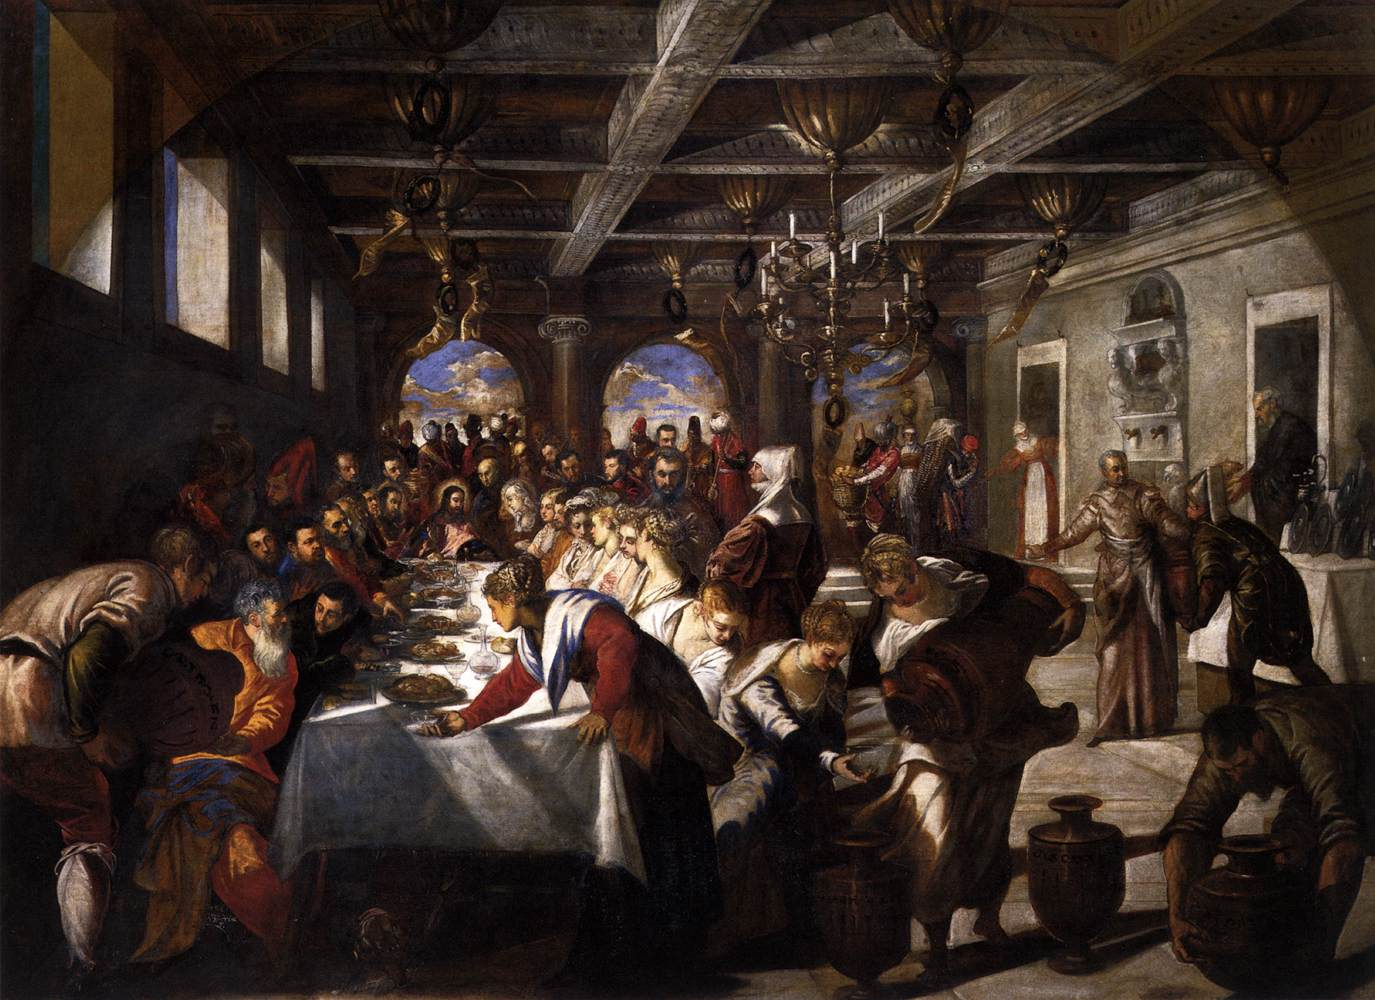
\includegraphics[angle=90, width=1\textwidth]{images/illustrations/tintorettomarriage.jpeg}
\end{center}
\vfill\vfill

%%%%%%%%%% Appendix %%%%%%%%%%
\pagenumbering{gobble}
\part*{\textsc{Appendix}}
	\markboth{Appendix}{Appendix}
	\addcontentsline{toc}{part}{Appendix}
\thispagestyle{empty}
  \mbox{}
  \newpage

\pagenumbering{roman}
\chapter*{The Greek Alphabet \\ \large From Alpha to Omega}
  \markboth{The Greek Alphabet}{The Greek Alphabet}
  \addcontentsline{toc}{chapter}{The Greek Alphabet}
  
As this edition of John's Apocalypse contains not only my own translation but also the original Greek text, I believed it to be helpful to include herein a small overview of the various letters of the Greek alphabet and their equivalent transliteration in English. 

As this is merely supposed to be a short guideline for the slightly-above-casual reader unaccustomed to the Greek alphabet — or, perhaps, having rudimentary knowledge thereof —, I decided against fully-fledged explanations of the various breathings and accents, and I also decided against describing their pronunciations; for, indeed, there exist such a large number of varying ways of pronouncing the Ancient Greek language that showcasing them all herein would not be possible. 

Instead, I recommend this table to be used simply as a quick reference guide for those who wish to read a handful of words in the Greek text — but are, due to their never having learnt the alphabet, unable to do so on their own —, or for those who have begun studying Greek only recently and still require help in reading the glyphs. 
  
\begin{center}
	\begin{longtable}{p{0.45\linewidth} | p{0.45\linewidth}}
    	Greek Letter & Transliteration \\ [0.5ex]
    	
    \hline\hline
    Α, α & a \\
    \hline
    Β, β & b \\
    \hline
    Γ, γ & g \\
    \hline
    Δ, δ & d \\
    \hline
    Ε, ε & e \\
    \hline
    Ζ, ζ & z \\
    \hline
    Η, η & \=e \\
    \hline
    Θ, θ & th \\
    \hline
    Ι, ι & i \\
    \hline
    Κ, κ & k \\
    \hline
    Λ, λ & l \\
    \hline
    Μ, μ & m \\
    \hline
    Ν, ν & m \\
    \hline
    Ξ, ξ & x \\
    \hline
    Ο, ο & o \\
    \hline
    Π, π & p \\
    \hline
    Ρ, ρ & r \\
    \hline
    Σ, σ, ς & s, z \\
    \hline
    Τ, τ & t \\
    \hline
    Υ, υ & u, y \\
    \hline
    Φ, φ & f, ph \\
    \hline
    Χ, χ & kh, ch \\
    \hline
    Ψ, ψ & ps \\
    \hline
    Ω, ω & \=o \\
    \hline
	\end{longtable}
\end{center}
\chapter*{Further Reading \\ \large Whereto Now?}
  \markboth{Further Reading}{Further Reading}
  \addcontentsline{toc}{chapter}{Further Reading}
  
If this book has fuelled your desire to learn not only more about the Apocalypse of John and the Bible in general, but also the Ancient Greek language, I believe the following section might be of interest to you. For I have, over the course of my studying Ancient Greek, made good use of a rather large repertoire of various resources and would like to showcase those I believe to be most helpful. 

First and foremost, I highly recommend JACT's ``Reading Greek'' series for commencing your study of the Ancient Greek language. In this series, as opposed to more traditional grammar books, you learn the language by reading as much as possible as soon as possible — as, indeed, the name should have revealed. If you do decide to get yourself a copy of the \textit{Reading Greek} series, I also highly recommend the Italian edition of ``Athenaze'', as it contains a very large amount of beginner-friendly prose. I cannot, however, recommend \textit{Athenaze} as one's only method of learning the language, as it does contain a not insignificant amount of Italian — thus, unless you speak Italian reasonably well, I can only recommend this book as a pairing to the aforementioned \textit{Reading Greek} series.

If you wish to continue reading the New Testament in its original language, my personal favourite is “The Greek New Testament: A Reader's Edition”. It contains not only the entirety of the Greek New Testament and an Greek-English dictionary at the back, but also parsed vocabulary at the bottom of the page; that way, the reader is required to learn only those words that occur thirty times or more in the New Testament — the remaining ones can be found at the bottom of the page. Additionally, all vocabulary is parsed, so that the reader can immediately identify what the conjugation of a particular verb or irregular noun is. Its ISBN is 978-3-438-05168-4.

There also exists a reader’s edition of the Greek Old Testament — which is also known as the “Septuagint(a)” — in a similar style as the above-mentioned New Testament reader; it is called “Septuaginta: A Reader's Edition”. In this rather extensive work — comprised not of one, but two volumes with over 1000 pages each —, you find the entirety of the Old Testament — including a handful of apocrypha —, a Greek-English dictionary and parsed vocabulary at the bottom of each page. It is a rather hefty investment, but the exceptional quality makes it, in my opinion, worthwhile. Its ISBN is 978-3-438-05190-5.

But there exist not only books that may aid you in your journey of studying the Greek Bible — and Greek in general —, but there also exists a rather considerable repository of resources that you can find on the Web. My own website, for example, \url{ancient-greek.net} contains a lot of information on Ancient Greek, how to study it and lots of reviews of various resources I use for learning the language. I highly recommend taking a look at it, as you can not only find aforesaid information thereon, but also links to a myriad of other helpful sites. 

And last — but most definitely not least —, I highly recommend you take a look at the other books in my New Testament Translation Series.

\chapter*{Afterword}
  \markboth{Afterword}{Afterword}
  \addcontentsline{toc}{chapter}{Afterword}

I thank you greatly for having read through the entirety of the book and hope that you enjoyed yourself whilst doing so. I have, to the best of my abilities, tried doing the original work justice, so that not only the unique and colourful manner in which John wrote his Revelation is translated properly, but also so that it becomes accessible and enjoyable for as many people as possible.

\bigskip\bigskip

\epigraph{\uppercase{αὐτῷ ἡ δόξα καὶ τὸ κράτος εἰς τοὺς αἰῶνας τῶν αἰώνων· ἀμήν.}}{Rev. 1:6}

\end{document}